% !TeX program = xelatex
\documentclass[UTF8,fontset=fandol,10pt,a4paper]{ctexart}
\usepackage[left=22mm,right=22mm,top=23mm,bottom=22mm,headheight=14pt]{geometry}
\usepackage{fontspec}
\setmainfont{TeX Gyre Heros}
\setsansfont{TeX Gyre Heros}
\setmonofont{Latin Modern Mono}
\renewcommand{\familydefault}{\sfdefault}
\usepackage[table]{xcolor}
\usepackage{graphicx,tikz}
\usetikzlibrary{arrows.meta,positioning,fit,backgrounds,calc}
\usepackage{booktabs,tabularx,array,enumitem,float,caption,fancyhdr,hyperref}
\definecolor{blue}{HTML}{2869A9}
\definecolor{ink}{HTML}{293340}
\definecolor{muted}{HTML}{647181}
\definecolor{line}{HTML}{C5D4E2}
\definecolor{pale}{HTML}{F0F5FA}
\definecolor{warm}{HTML}{FFF7E9}
\hypersetup{colorlinks=true,urlcolor=blue,linkcolor=blue,pdftitle={Redflag RHI 与 Vulkan 接入设计},pdfauthor={Redflag}}
\color{ink}
\setlength{\parindent}{0pt}
\setlength{\parskip}{6pt}
\linespread{1.16}
\setlist[itemize]{leftmargin=1.5em,itemsep=2pt,topsep=3pt}
\setlist[enumerate]{leftmargin=1.8em,itemsep=3pt,topsep=3pt}
\renewcommand{\arraystretch}{1.38}
\newcolumntype{Y}{>{\raggedright\arraybackslash}X}
\newcolumntype{L}[1]{>{\raggedright\arraybackslash}p{#1}}
\ctexset{section={format=\Large\bfseries\color{blue},beforeskip=16pt,afterskip=8pt},subsection={format=\large\bfseries\color{blue},beforeskip=11pt,afterskip=5pt}}
\captionsetup{font=small,labelfont=bf,textfont={color=muted},skip=7pt}
\pagestyle{fancy}\fancyhf{}
\fancyhead[L]{\small\color{muted}Redflag · RHI / Vulkan · 设计方案}
\fancyhead[R]{\small\color{muted}2026-11-21}
\fancyfoot[C]{\small\color{muted}\thepage}
\renewcommand{\headrulewidth}{0pt}
\newcommand{\note}[1]{{\small\color{muted}#1\par}}
\newcommand{\code}[1]{{\small\texttt{#1}}}
\newcommand{\ruleline}{\par\vspace{4pt}{\color{line}\hrule}\vspace{8pt}}
\newcommand{\source}[2]{{\small\href{#1}{[#2]}}}
\tikzset{
 module/.style={draw=line,fill=pale,rounded corners=2pt,align=center,inner sep=7pt,text width=3.8cm,minimum height=1.15cm,font=\small},
 smallbox/.style={module,text width=2.55cm,minimum height=.95cm,font=\footnotesize},
 wide/.style={module,text width=9.5cm},
 planned/.style={module,fill=warm,dashed},
 flow/.style={-{Stealth[length=2mm]},draw=muted,line width=.65pt},
 own/.style={flow,dashed},
 label/.style={font=\scriptsize,fill=white,inner sep=2pt,text=muted}}

\geometry{a4paper,landscape,left=17mm,right=17mm,top=14mm,bottom=14mm}
\hypersetup{pdftitle={维修站回收场 · 场景概念与地编},pdfauthor={Redflag}}
\definecolor{ochre}{HTML}{995A2B}
\definecolor{steel}{HTML}{3B5261}
\definecolor{sand}{HTML}{EBDCC8}
\fancyhead[L]{}\fancyhead[R]{}\fancyfoot[C]{}
\fancyfoot[R]{\small\color{muted}Redflag\hspace{1em}\thepage}
\setlength{\parindent}{2\ccwd}\setlength{\parskip}{4pt}
\ctexset{section={format=\Large\bfseries\color{steel},afterindent=true,beforeskip=1pt,afterskip=4pt}}
\newcommand{\figtext}[1]{\par\noindent{\small\color{muted}#1}\par}
\begin{document}
\section*{维修站回收场}
站在西侧入口，最先看见的是半开的棚门。棚里亮着一盏灯，下面停着等待维修的发电机。通向棚门的路保留了一段旧路面，两侧才是拆下来的轮毂、货架和零件。玩家即使还没有读任务提示，也有一个可以先走过去看看的地方。

\begin{center}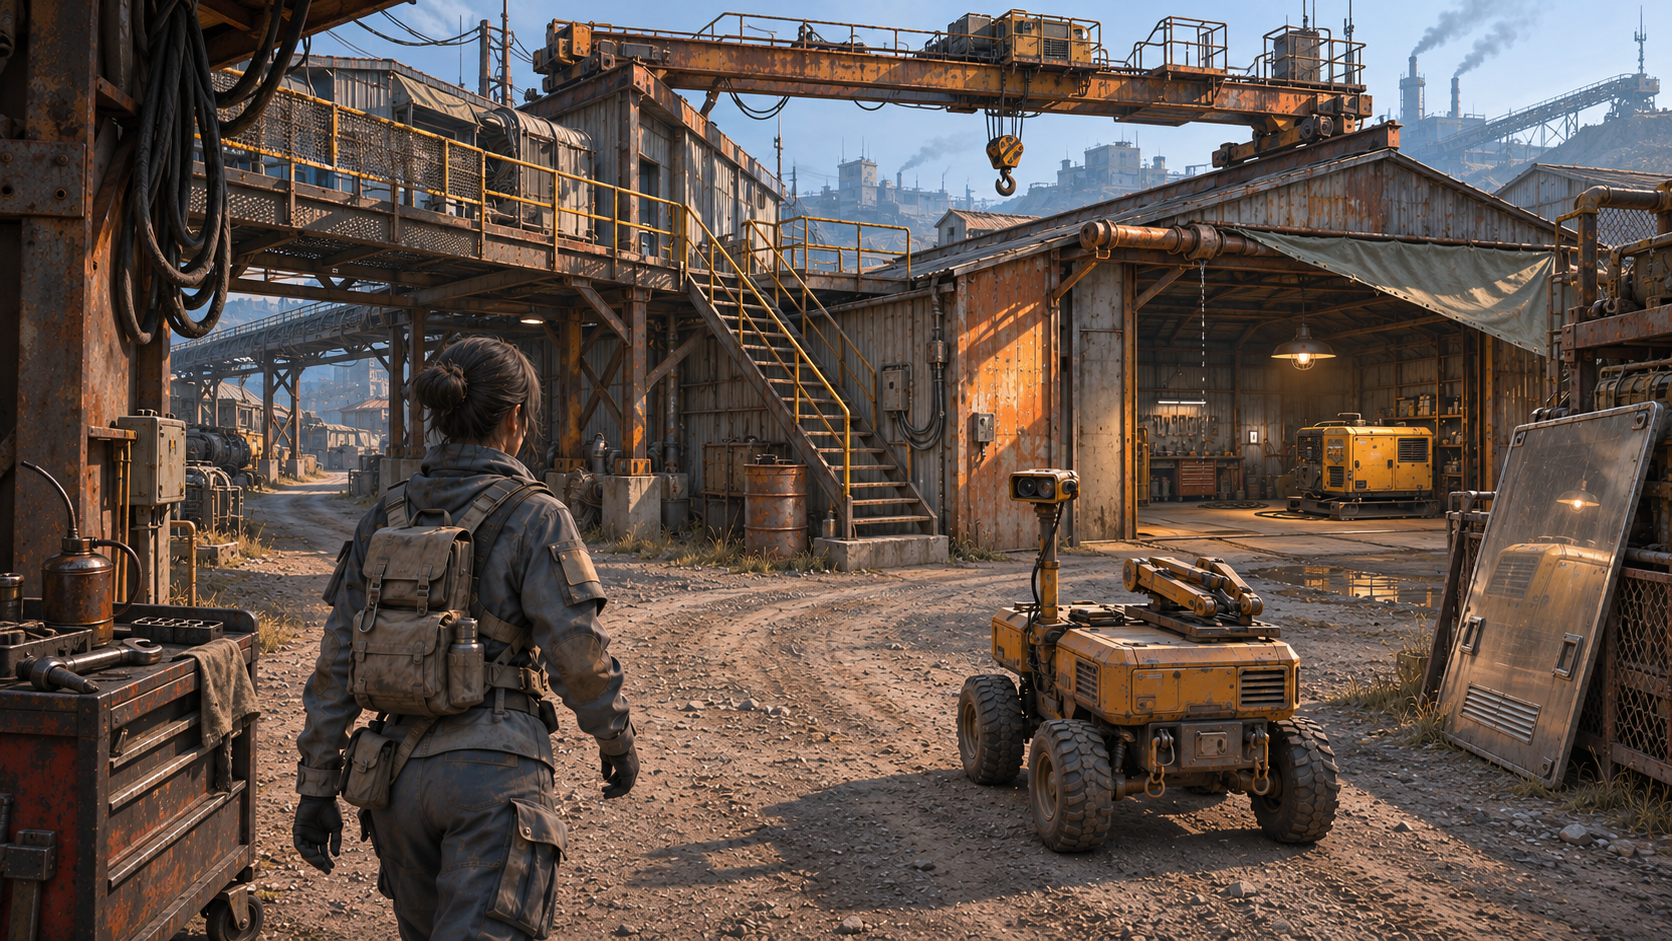
\includegraphics[width=.90\linewidth,height=126mm,keepaspectratio]{figures/yard-crane.png}\end{center}
\figtext{场景概念图，由 ImageGen 为本项目生成。以暖色回收场为日间目标，远处厂房留出一层灰蓝色。玩家的直立轮廓和瓦特贴近地面的车身，在去掉颜色以后仍应当容易区分。游戏目前以同骨架的蓝灰、赭色两名机器人试玩，图中的轮式伙伴仍是造型目标。}

\newpage
\section*{从入口到维修棚}
从玩家的位置到发电机约十四米。正面能看见棚门，另一条路沿着工具架绕到棚边，中途可以先取补给。侧路值得走，是因为它经过玩家当下可能需要的东西。两条路最后都回到同一个地标，转身找队友时也能认出自己的方位。

\begin{center}
\begin{tikzpicture}[x=.78cm,y=.69cm,font=\sffamily\small,>=Stealth]
\fill[fill=sand!48,draw=ochre!50,rounded corners=3pt] (-10,-5.8) rectangle (10,5.8);
\fill[steel!65] (-8.5,3.1) rectangle (-5.2,5.25);
\node[text=white] at (-6.85,4.2){西棚货柜};
\fill[steel!65] (5.0,3.55) rectangle (8.8,5.35);
\node[text=white] at (6.9,4.45){东棚货柜};
\fill[steel!17] (-7.7,-5.55) rectangle (-4.2,-4.35);
\node at (-5.95,-4.95){货架、油桶};
\draw[ochre,thick,dashed,rounded corners] (5,-3.75) rectangle (9.2,.45);
\node[anchor=south,text=ochre] at (7.1,.45){铁皮维修棚};
\draw[steel,line width=2.4pt,-{Stealth[length=3mm]}] (-6.9,-1.4) .. controls (-4.6,.25) and (1.2,.3) .. (6.55,-1.2);
\draw[ochre,thick,dashed,-{Stealth[length=3mm]}] (-6.9,-1.5) .. controls (-5,-2.5) and (-4.15,-2.65) .. (-3.4,-2.15)
 .. controls (-1.8,-3.9) and (3.2,-3.7) .. (6.8,-1.7);
\foreach \x/\y/\label in {-6.9/-1.4/玩家,-5.2/.6/瓦特,7/-1.4/发电机,-3.4/-2.15/急救工具箱}{
 \fill[steel] (\x,\y) circle (2.7pt);
 \node[anchor=south,fill=sand!40,inner sep=1.5pt] at (\x,\y+.12){\label};}
\draw[steel,|-|] (-9.2,-3.6)--(-7.2,-3.6);
\node[above,scale=.82] at (-8.2,-3.6){2 米};
\node[anchor=west,text=steel] at (-9.8,6.18){西侧入口};
\node[anchor=east,text=steel] at (9.8,6.18){东侧工位};
\end{tikzpicture}
\end{center}
\figtext{样板平面。人物、物品和货柜据场景配置定位。实线和虚线给出待试玩的两种走法，棕色虚线框标出实机关卡里的铁皮棚。图只画可行走的维修场；远处的厂房用于交代环境。}

看概念图时，先把它缩到半个屏幕：行车的横梁与棚顶在远景上留下一条清楚的边，暖灯下面有机器的暗面。放回第三人称镜头时再查同一件事。货架可以堆密一点，但不能把玩家眼前的门遮住；瓦特绕到侧面后，也要能从货柜的轮廓里分出来。

\newpage
\section*{路肩、车道与采石坡}
\begin{center}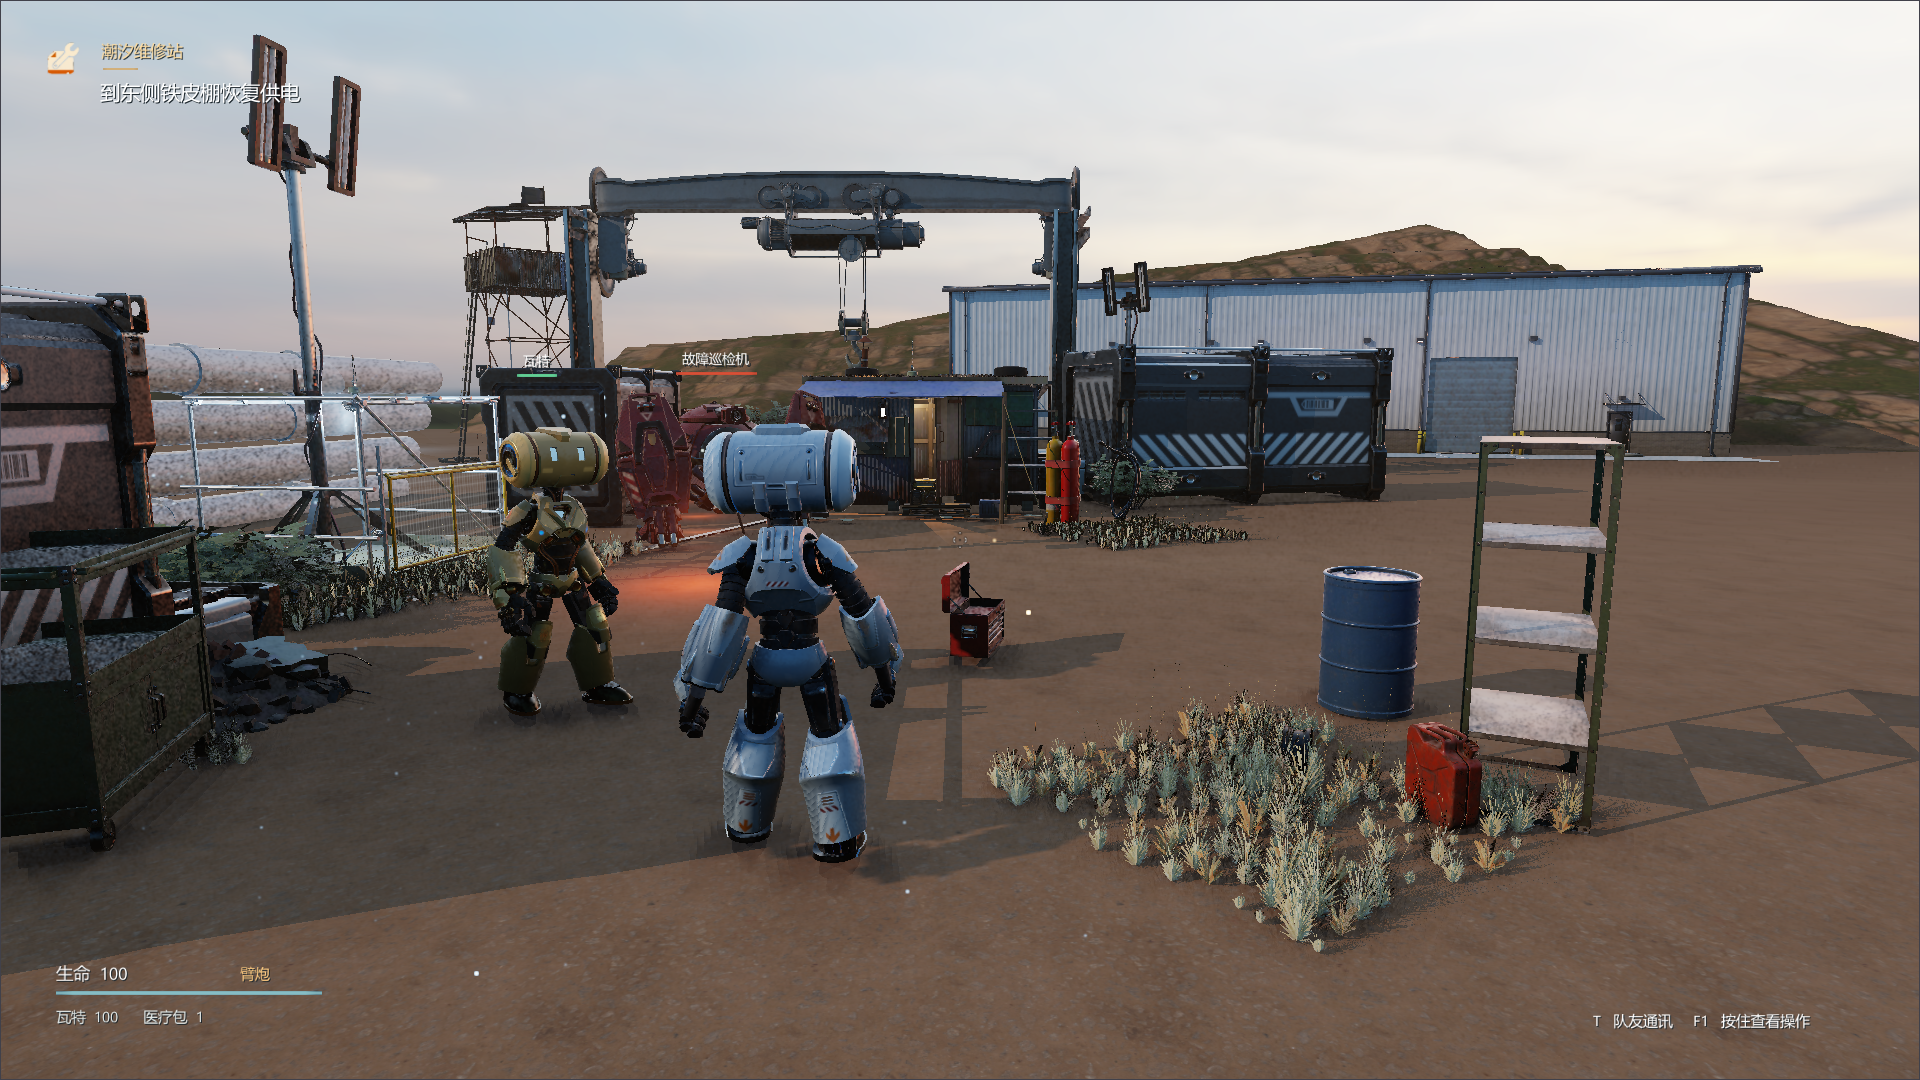
\includegraphics[width=.87\linewidth,height=112mm,keepaspectratio]{../../../output/validation/watt-station/yard-instrument-hud.png}\end{center}
\figtext{正式 Vulkan 游戏，西侧出生点，1920 × 1080。蓝灰色是玩家，左边的赭色角色是瓦特。压实的车道一直通向中央铁皮棚。左上方的值班塔、右侧的浅色仓库和后方岩坡分别处在不同距离。}

砂石路和采石坡用了两种不同尺度的照片。走近工具车时，能看清碎石之间的间隙，所以脚下这张材质每两米重复一次。看远处山体时，重要的是辨认成片裸岩和草地。山坡改用了航拍地表，每四十二米重复一次。起伏则直接读取高程图，来自美国地质调查局在盐湖城一带的测量。这里为关卡压缩了水平和竖直尺度。

搬运设备的车道留空，草丛沿器材脚下、路缘和坡脚分布。近处可以借推车认路，到了棚门依然能借塔看清来时的方向。编辑时移动其中一簇草，只会改变这个位置的摆放；相同的草模型可以在别处继续使用。

\figtext{素材：\href{https://polyhaven.com/a/gravel_road}{Gravel Road}、\href{https://polyhaven.com/a/rocky_terrain}{Rocky Terrain}（Amal Kumar，CC0）；\href{https://tevy.dev/models/savanna-grass-patch}{旱草}、\href{https://tevy.dev/models/watchtower-scrap}{值班塔}、\href{https://tevy.dev/models/warehouse}{仓库}（tevy，CC0）。}

\clearpage
\section*{维修棚的工作灯}
\noindent\begin{minipage}[t]{.49\linewidth}\vspace{0pt}
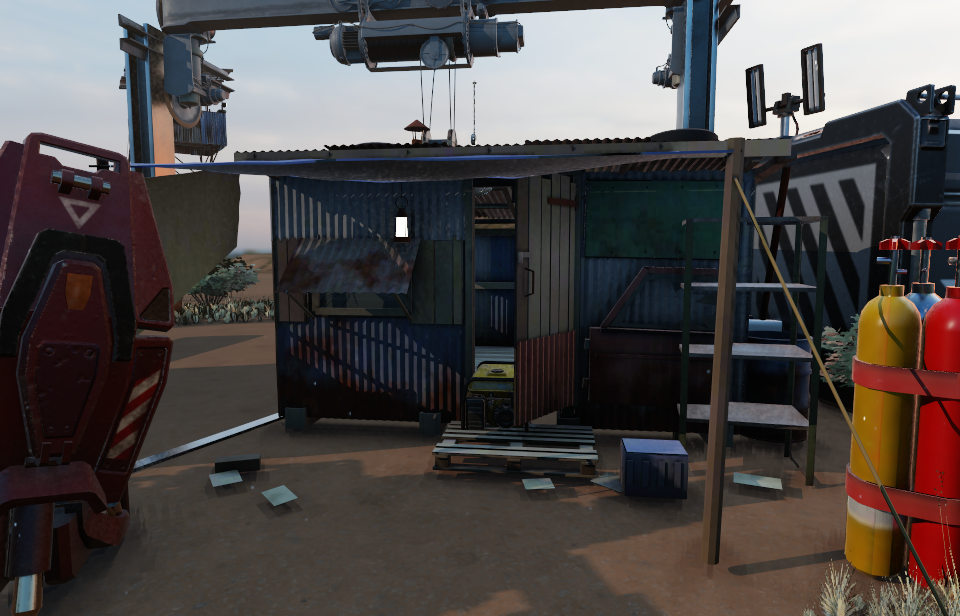
\includegraphics[width=\linewidth]{../../../output/validation/watt-station/workshop-light/off.png}
\figtext{关灯。观察棚顶下面的门板和发电机外壳。}
\end{minipage}\hfill\begin{minipage}[t]{.49\linewidth}\vspace{0pt}
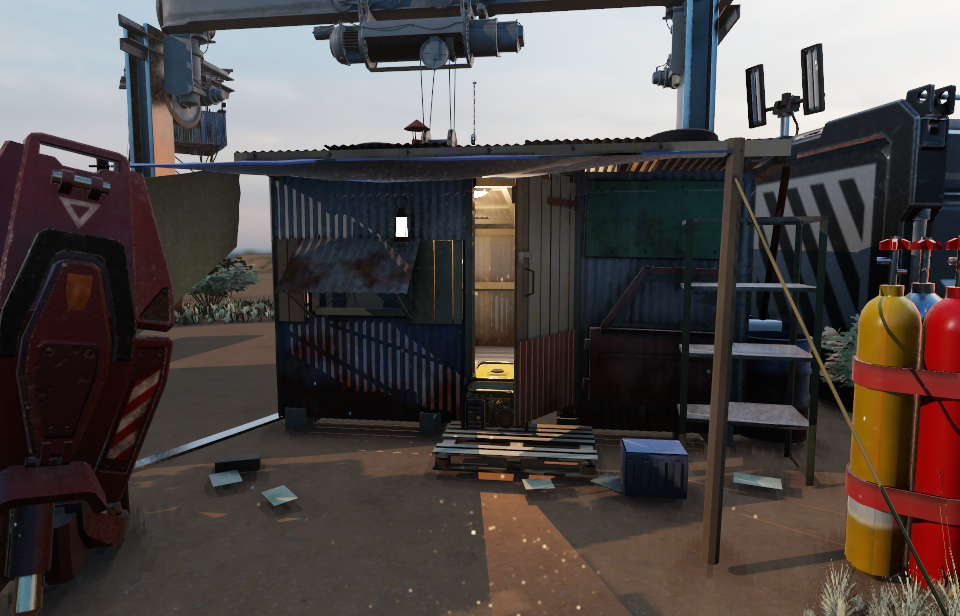
\includegraphics[width=\linewidth]{../../../output/validation/watt-station/workshop-light/on.png}
\figtext{开灯。同一相机和曝光，门内亮起一片暖光。}
\end{minipage}

在仓库前停住，最容易认出的光来自铁皮棚的门口。灯泡吊在发电机上方，暖光落在门内侧和机器外壳上。另一盏冷色灯靠近左侧管廊，照亮检修台。两处灯都保存在场景里，移动灯具时应一并移动对应的点光源。

瓦特进入工位时，可以读取地编写的工位说明，也能查询关联灯的实际强度。在角色的观察记录里，这两条信息有各自的来源。灯开着也可能被墙挡住，要知道瓦特能否从当前角度看见它，就需要从瓦特眼睛的位置拍一张图。

两张图来自 RenderDoc。在图像中央取宽、高各一半的区域，用同一批像素计算显示变换前的平均亮度。关灯时为 0.05024，开灯时为 0.14421，约为原先的 2.87 倍。逐像素对照表面颜色，两帧完全相同。这次比较测的是工作灯照亮了多少，镜面多次反射另用每次只改变反射次数的实验验证，见《渲染公式与实现》中的镜面反射一节。

\vspace{5mm}
\figtext{铁皮棚和脚手架见\href{https://tevy.dev/models/scrap-shanty}{tevy}，发电机见\href{https://polyhaven.com/a/portable_generator}{Poly Haven}，管廊和部件见\href{https://github.com/godotengine/tps-demo}{Godot 第三人称样例}。}

\clearpage
\section*{碎石路面的细节}
维修站的地面是一张平面，脚下的石块主要靠贴图表现。原先铺路时沿平面的两个方向放大一百倍，垂直方向却保留原尺寸，石面的法线随之变平。同一盏太阳下，有些本应朝向侧面的石棱和朝上的石面看起来几乎一样亮。让三个方向采用同一比例，既保留了平面的尺寸，也恢复了贴图中记录的石面朝向。

\begin{center}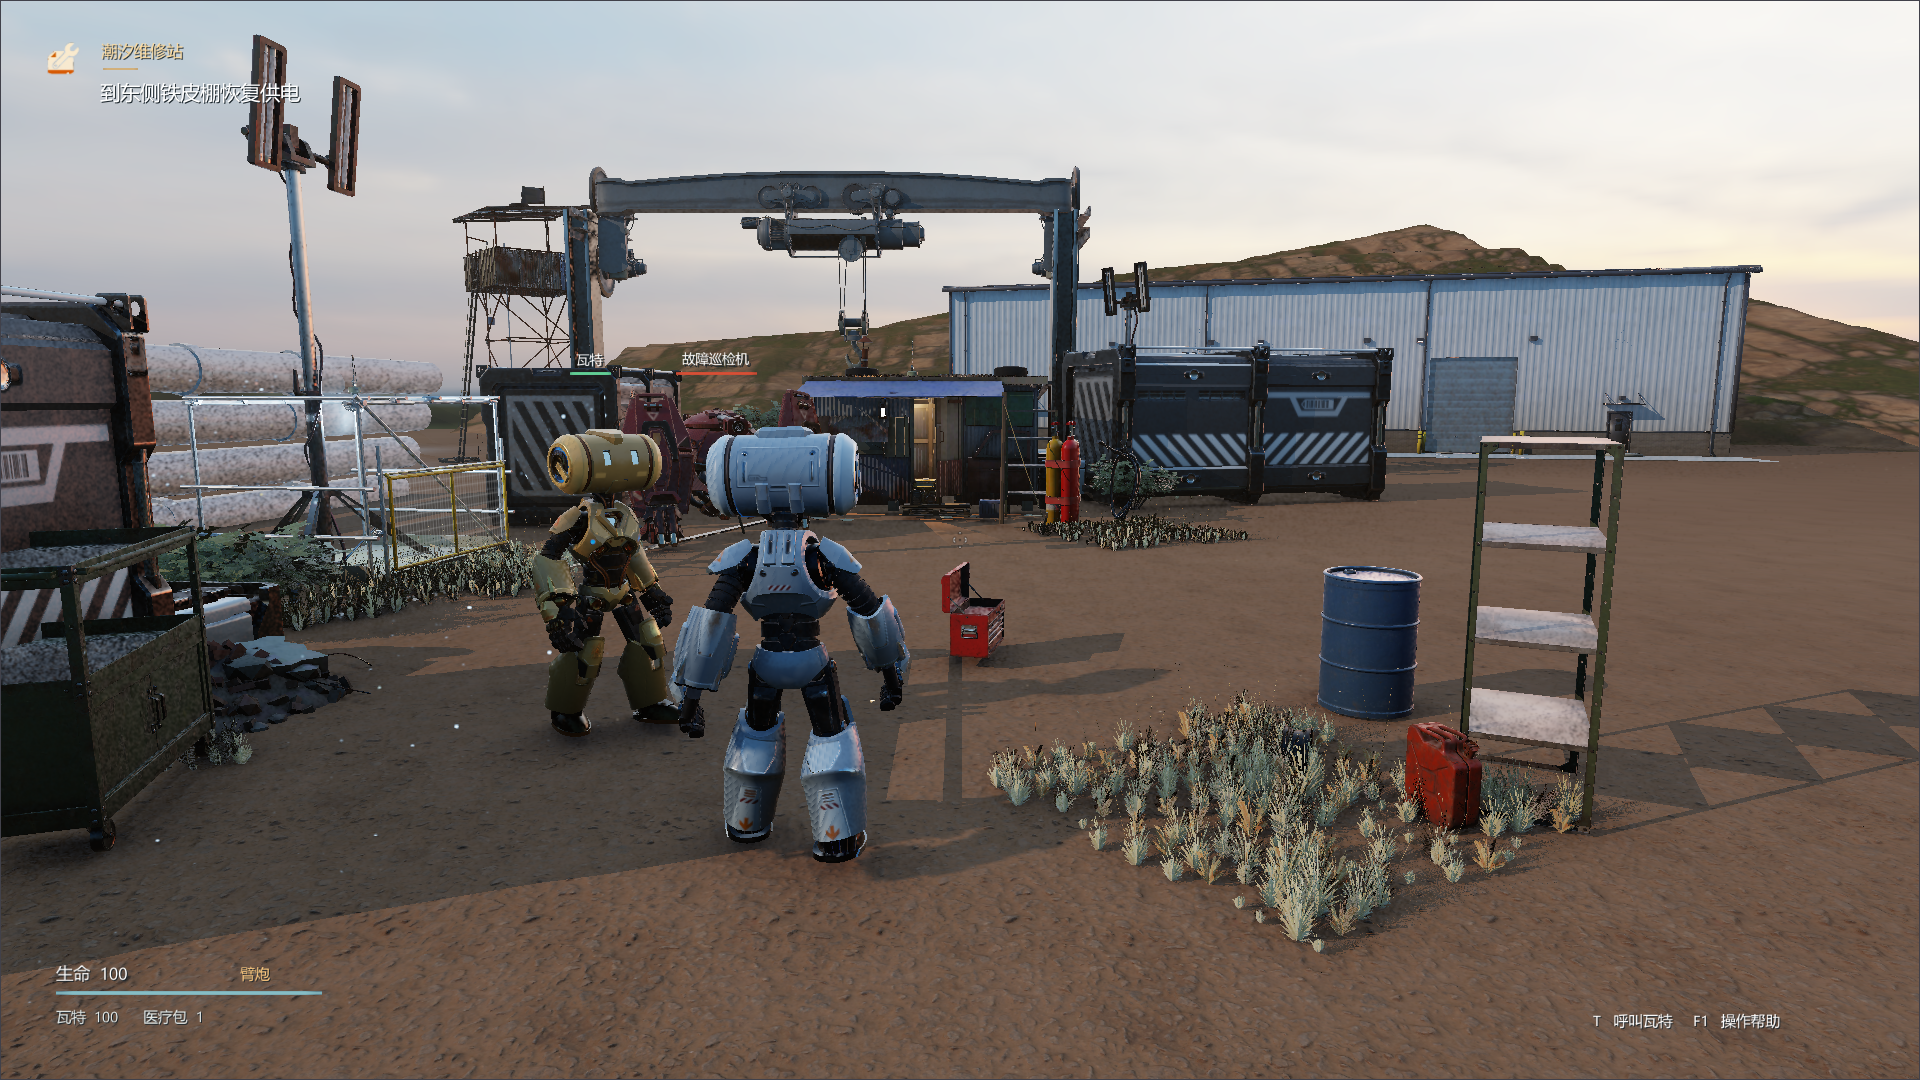
\includegraphics[width=.68\linewidth,height=80mm,keepaspectratio]{../../../output/validation/station-materials/spawn-current.png}\end{center}
\figtext{维修站游戏出生点，1920 × 1080 的 Vulkan 实机帧。近处能分清草叶之间的碎石，远处还能沿车道看到棚门。}

\begin{center}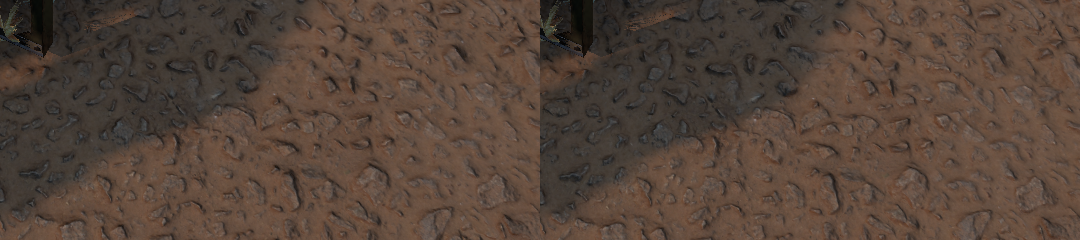
\includegraphics[width=.65\linewidth,height=35mm,keepaspectratio]{../../../output/validation/station-materials/gravel-normal-current-crop.png}\end{center}
\figtext{路肩的同机位局部。左图使用扫描法线，右图另外使用视差。斜看时，凸起石棱遮住了后面的一部分沟底。该次地面绘制的 GPU 中位耗时约从 150 增到 223 微秒。原始扫描见 \href{https://polyhaven.com/a/gravel_road}{Poly Haven}。}

\clearpage
\section*{工具架的漆面与备用轮毂}
\noindent\begin{minipage}[t]{.55\linewidth}\vspace{0pt}
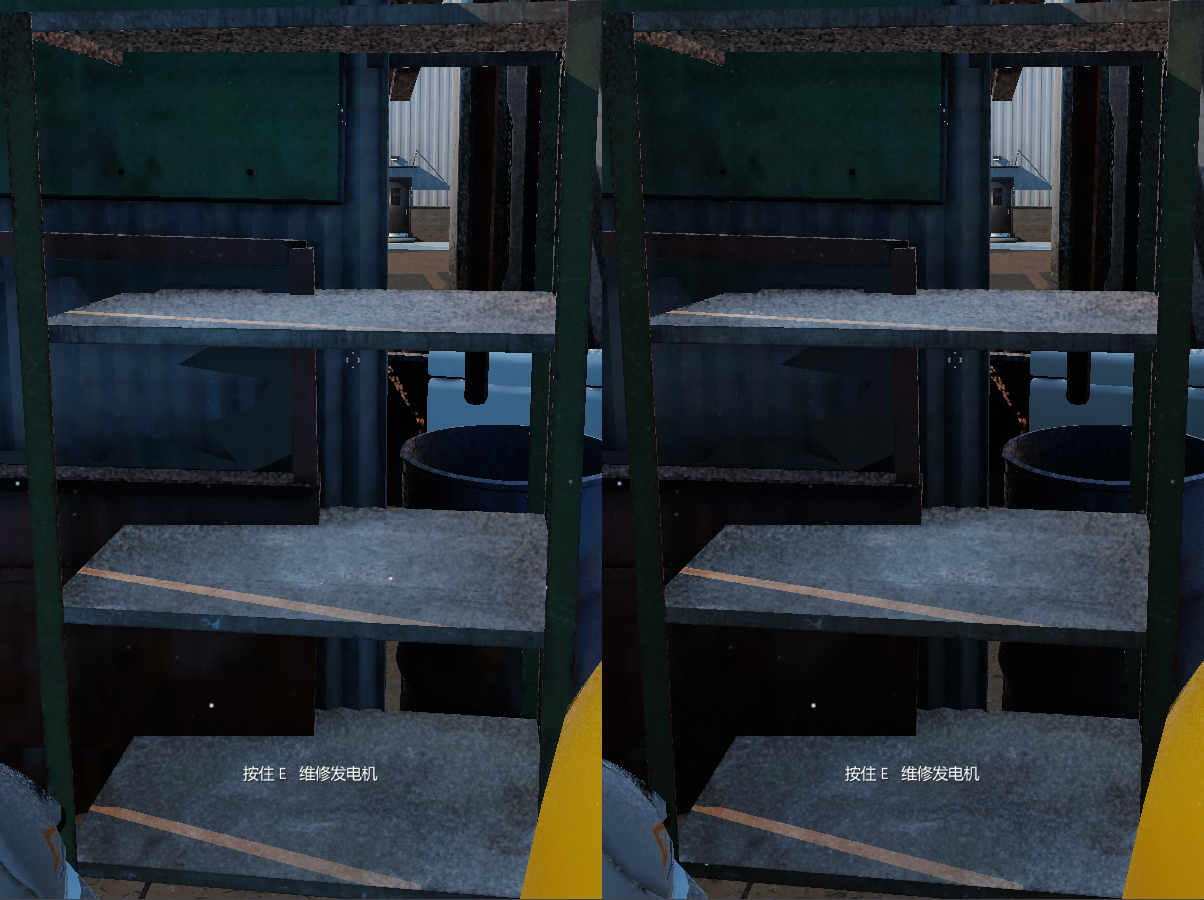
\includegraphics[width=\linewidth,height=96mm,keepaspectratio]{../../../output/validation/station-materials/rack-original-current-crop.png}
\figtext{同一工具架的局部，左为原始 1K，右为烘焙的 2K。找一条漆面上的浅色磨痕，对照边缘与受光。}
\end{minipage}\hfill\begin{minipage}[t]{.42\linewidth}\vspace{0pt}
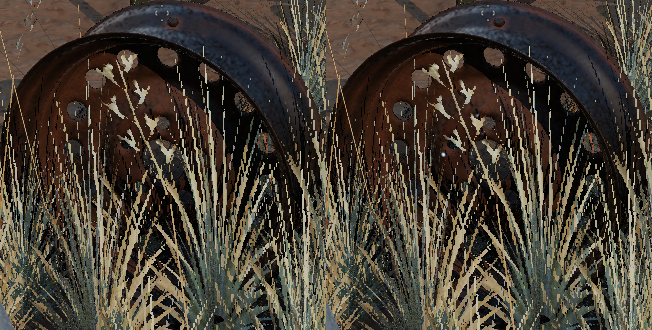
\includegraphics[width=\linewidth]{../../../output/validation/station-materials/rim-original-current-crop.png}
\figtext{同一轮毂，左侧保留原网格，右侧按扫描高度轻微移动顶点。轮辋边缘的变化需要靠近观察。}

工具架沿用原模型的贴图坐标。底色先换算成线性亮度再做平均；法线保存的是朝向，求平均后还要把向量长度恢复为 1。锈斑、油漆占的是底色和受光，架子边缘仍由网格决定。
\end{minipage}

工具架从作者的 4K 原图烘成 2K，远处同款仍使用内嵌的 1K。两张新图连同逐级缩小的副本，按每个像素四字节估算约占 42.67 MiB。交错回放两个版本，该架绘制的中位耗时为 49.23 与 49.02 微秒。轮毂使用同一作者配套的灰度高度图，移动顶点后近镜头下最大位移也只有约半个像素。这项处理适合近处可细看的零件。原始资产与授权见 \href{https://polyhaven.com/a/worn_metal_rack}{工具架}和\href{https://polyhaven.com/a/rusted_wheel_rim_01}{备用轮毂}。
\end{document}
